\subsection{HNSW算法多线程实现}

\subsubsection{实验设置}

本节针对分层小世界导航图(HNSW)算法的多线程实现进行性能分析。HNSW算法采用分层图结构进行近似最近邻搜索,具有优秀的搜索性能和召回率。

\paragraph{算法参数设置}
\begin{itemize}
    \item \textbf{M值}:图连接度参数,测试范围:8, 16, 24, 128, 256
    \item \textbf{efC值}:构造时的动态候选列表大小,测试范围:100, 150, 200
    \item \textbf{efS值}:搜索时的动态候选列表大小,测试范围:50, 100, 200, 300, 400, 500
\end{itemize}

\paragraph{实现版本}
\begin{itemize}
    \item \textbf{串行版本}:基础的单线程HNSW实现
    \item \textbf{OpenMP版本}:采用OpenMP并行化的多线程实现
\end{itemize}

\subsubsection{性能分析结果}

\paragraph{总体性能统计}

表~\ref{tab:hnsw_performance_stats}展示了不同实现的整体性能指标。

\begin{table}[htbp]
\centering
\caption{HNSW算法多线程实现性能统计}
\label{tab:hnsw_performance_stats}
\begin{tabular}{|c|c|c|c|c|c|c|}
\hline
\textbf{实现方式} & \multicolumn{3}{c|}{\textbf{加速比}} & \multicolumn{2}{c|}{\textbf{延迟(μs)}} & \textbf{平均召回率} \\
\cline{2-6}
 & 平均 & 最大 & 最小 & 平均 & 最小 & \\
\hline
串行版本 & 1.000 & 1.000 & 1.000 & 413.6 & 48 & 0.992 \\
OpenMP版本 & 0.661 & 1.547 & 0.115 & 708.2 & 49 & 0.992 \\
\hline
\end{tabular}
\end{table}

从统计结果可以看出,OpenMP并行化版本的平均性能反而比串行版本下降了约34\%,这表明HNSW算法的搜索过程存在并行化困难。

\paragraph{最佳配置分析}

表~\ref{tab:hnsw_best_configs}总结了各实现方式的最佳配置。

\begin{table}[htbp]
\centering
\caption{HNSW算法最佳配置分析}
\label{tab:hnsw_best_configs}
\begin{tabular}{|c|c|c|c|c|}
\hline
\textbf{实现方式} & \textbf{指标} & \textbf{配置} & \textbf{召回率} & \textbf{延迟(μs)} \\
\hline
\multirow{2}{*}{串行版本} & 最高召回率 & M=128, efC=100, efS=400 & 1.0000 & 709 \\
& 最低延迟 & M=8, efC=150, efS=50 & 0.9240 & 48 \\
\hline
\multirow{3}{*}{OpenMP版本} & 最高召回率 & M=128, efC=100, efS=400 & 1.0000 & 2843 \\
& 最低延迟 & M=8, efC=200, efS=50 & 0.9325 & 49 \\
& 最高加速比 & M=8, efC=200, efS=200 & 0.9920 & - \\
\hline
\end{tabular}
\end{table}

\paragraph{参数影响分析}

图~\ref{fig:hnsw_comprehensive}展示了HNSW算法的综合性能分析。

\begin{figure}[htbp]
\centering
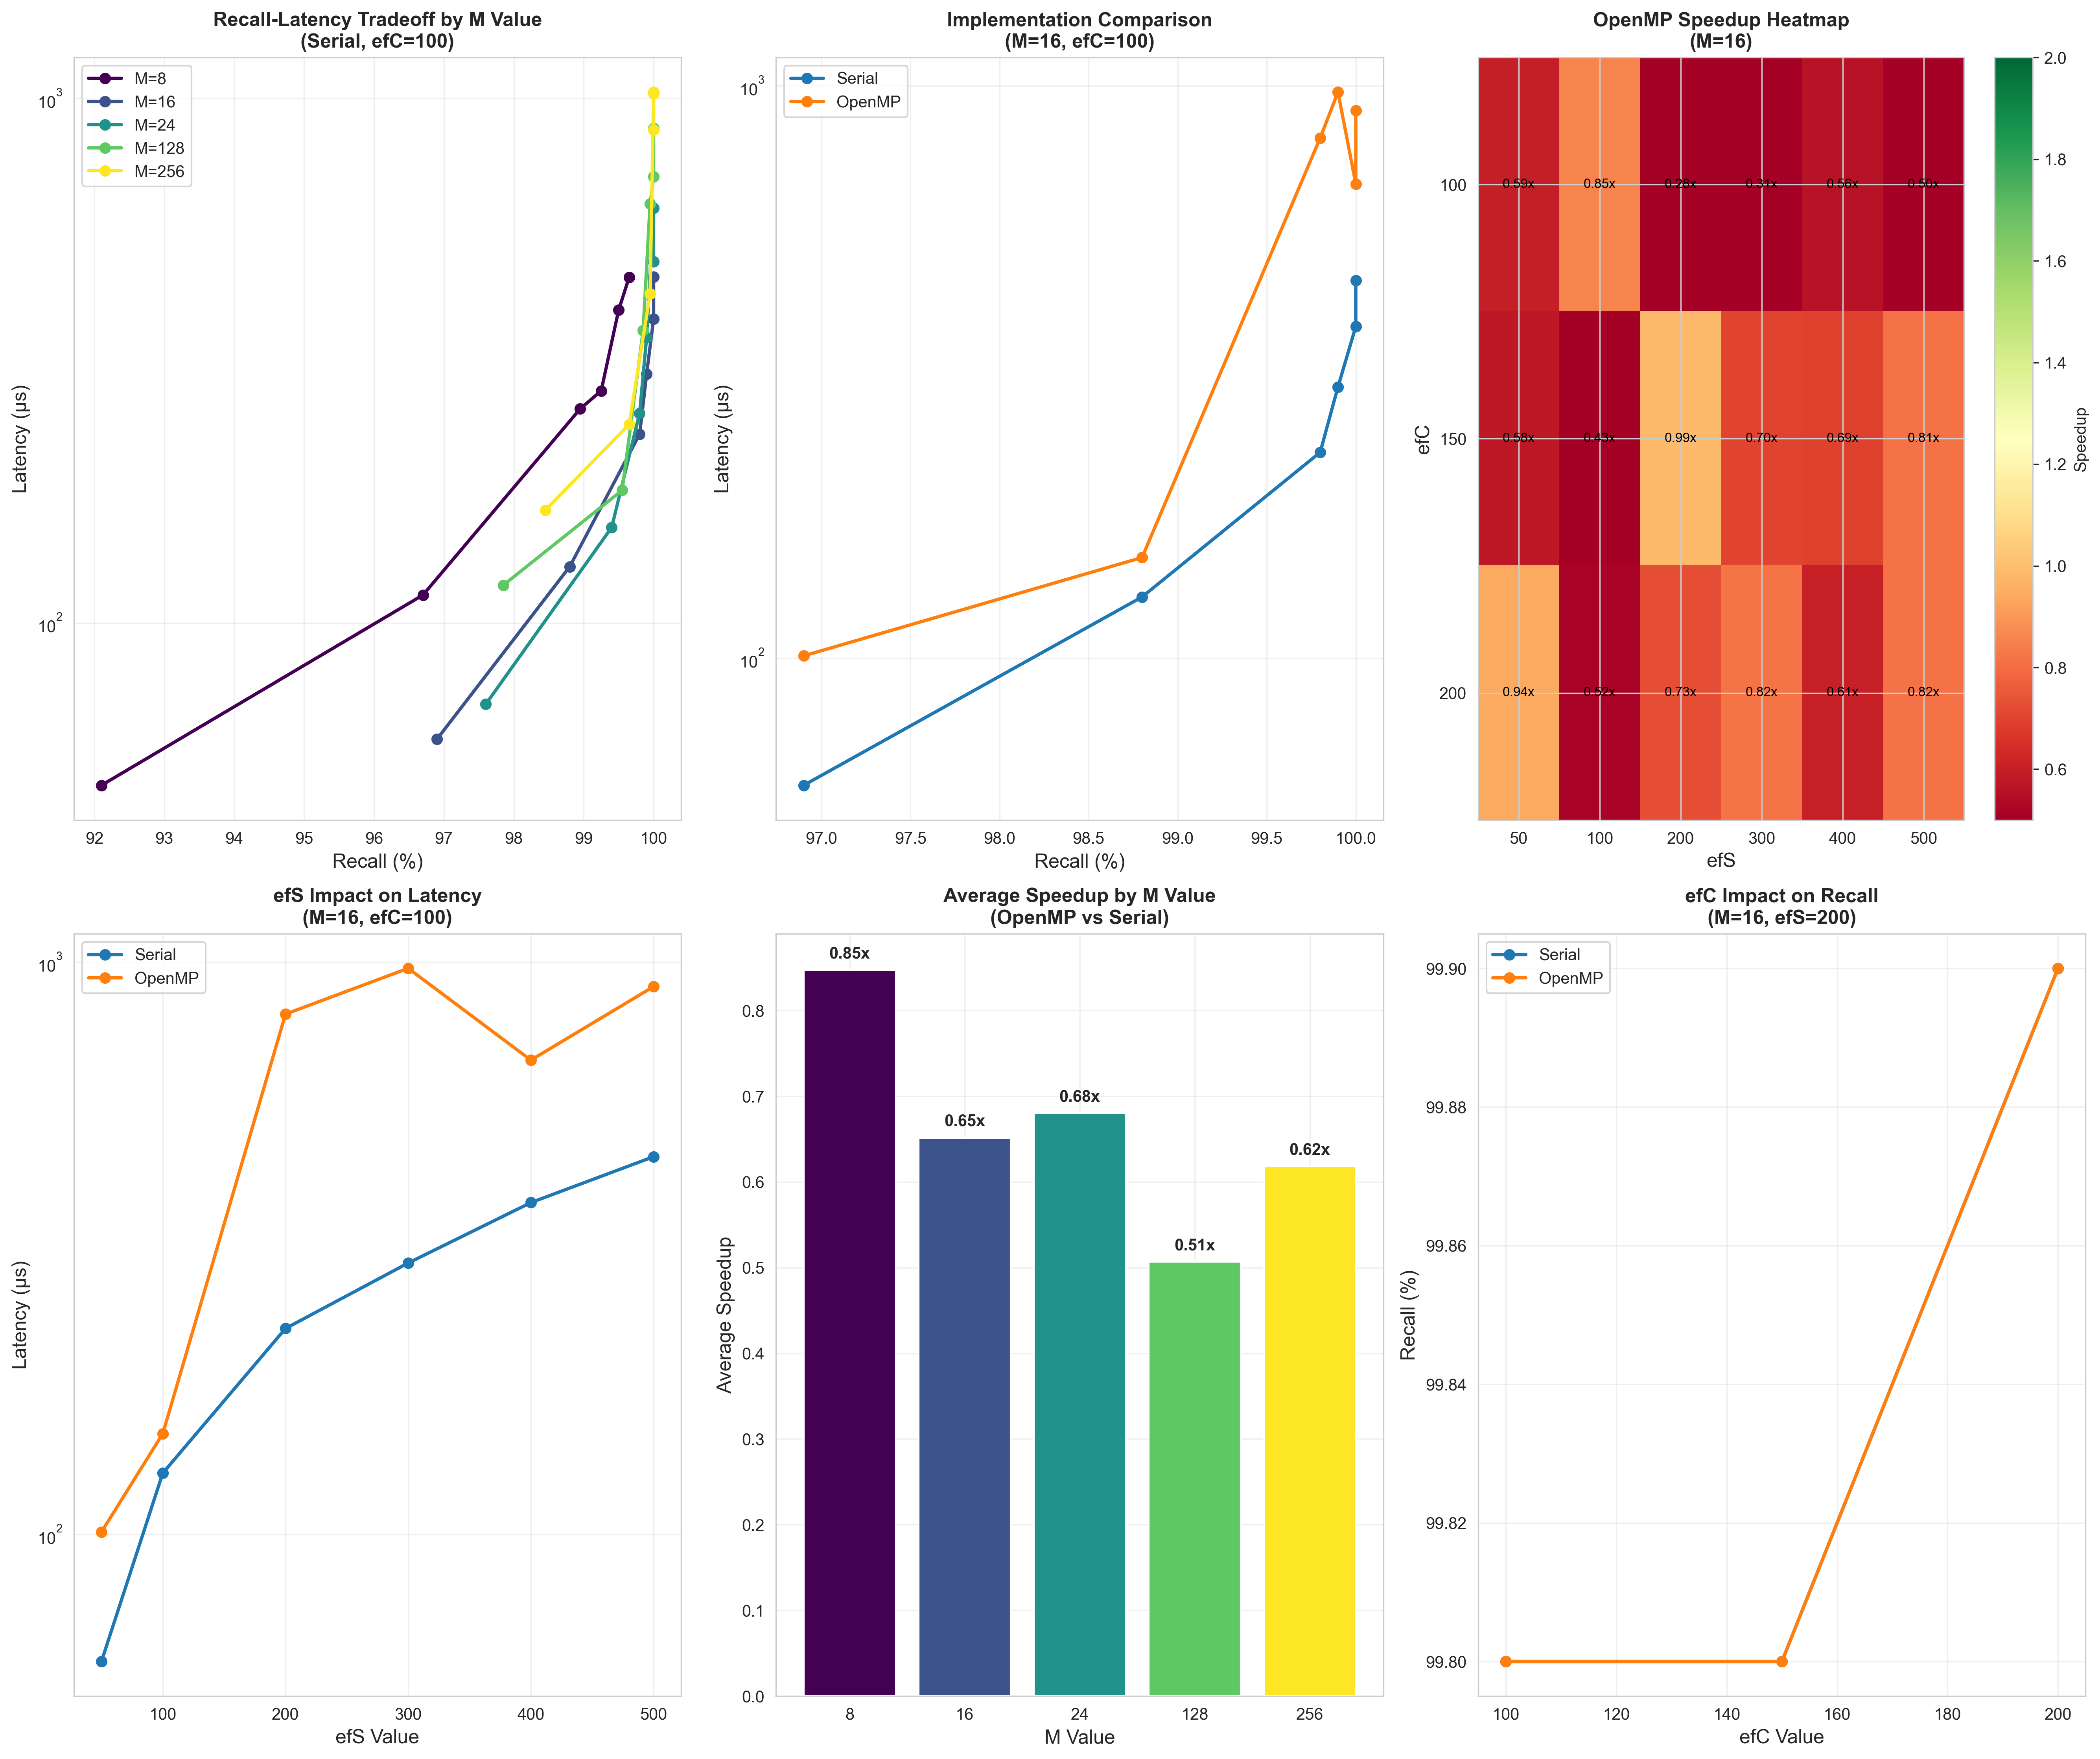
\includegraphics[width=\textwidth]{plots/hnsw_comprehensive_analysis_en.png}
\caption{HNSW算法多线程实现综合分析}
\label{fig:hnsw_comprehensive}
\end{figure}

从图中可以观察到:
\begin{enumerate}
    \item \textbf{M值对性能的影响}:较小的M值(8, 16)能够提供更好的延迟性能,而较大的M值(128, 256)有助于提高召回率
    \item \textbf{实现方式比较}:在大多数配置下,OpenMP版本的延迟都高于串行版本
    \item \textbf{加速比热力图}:只有在特定的参数组合下(如M=8的某些配置),OpenMP版本才能实现有限的加速效果
\end{enumerate}

图~\ref{fig:hnsw_parameter_sensitivity}进一步分析了参数敏感性。

\begin{figure}[htbp]
\centering
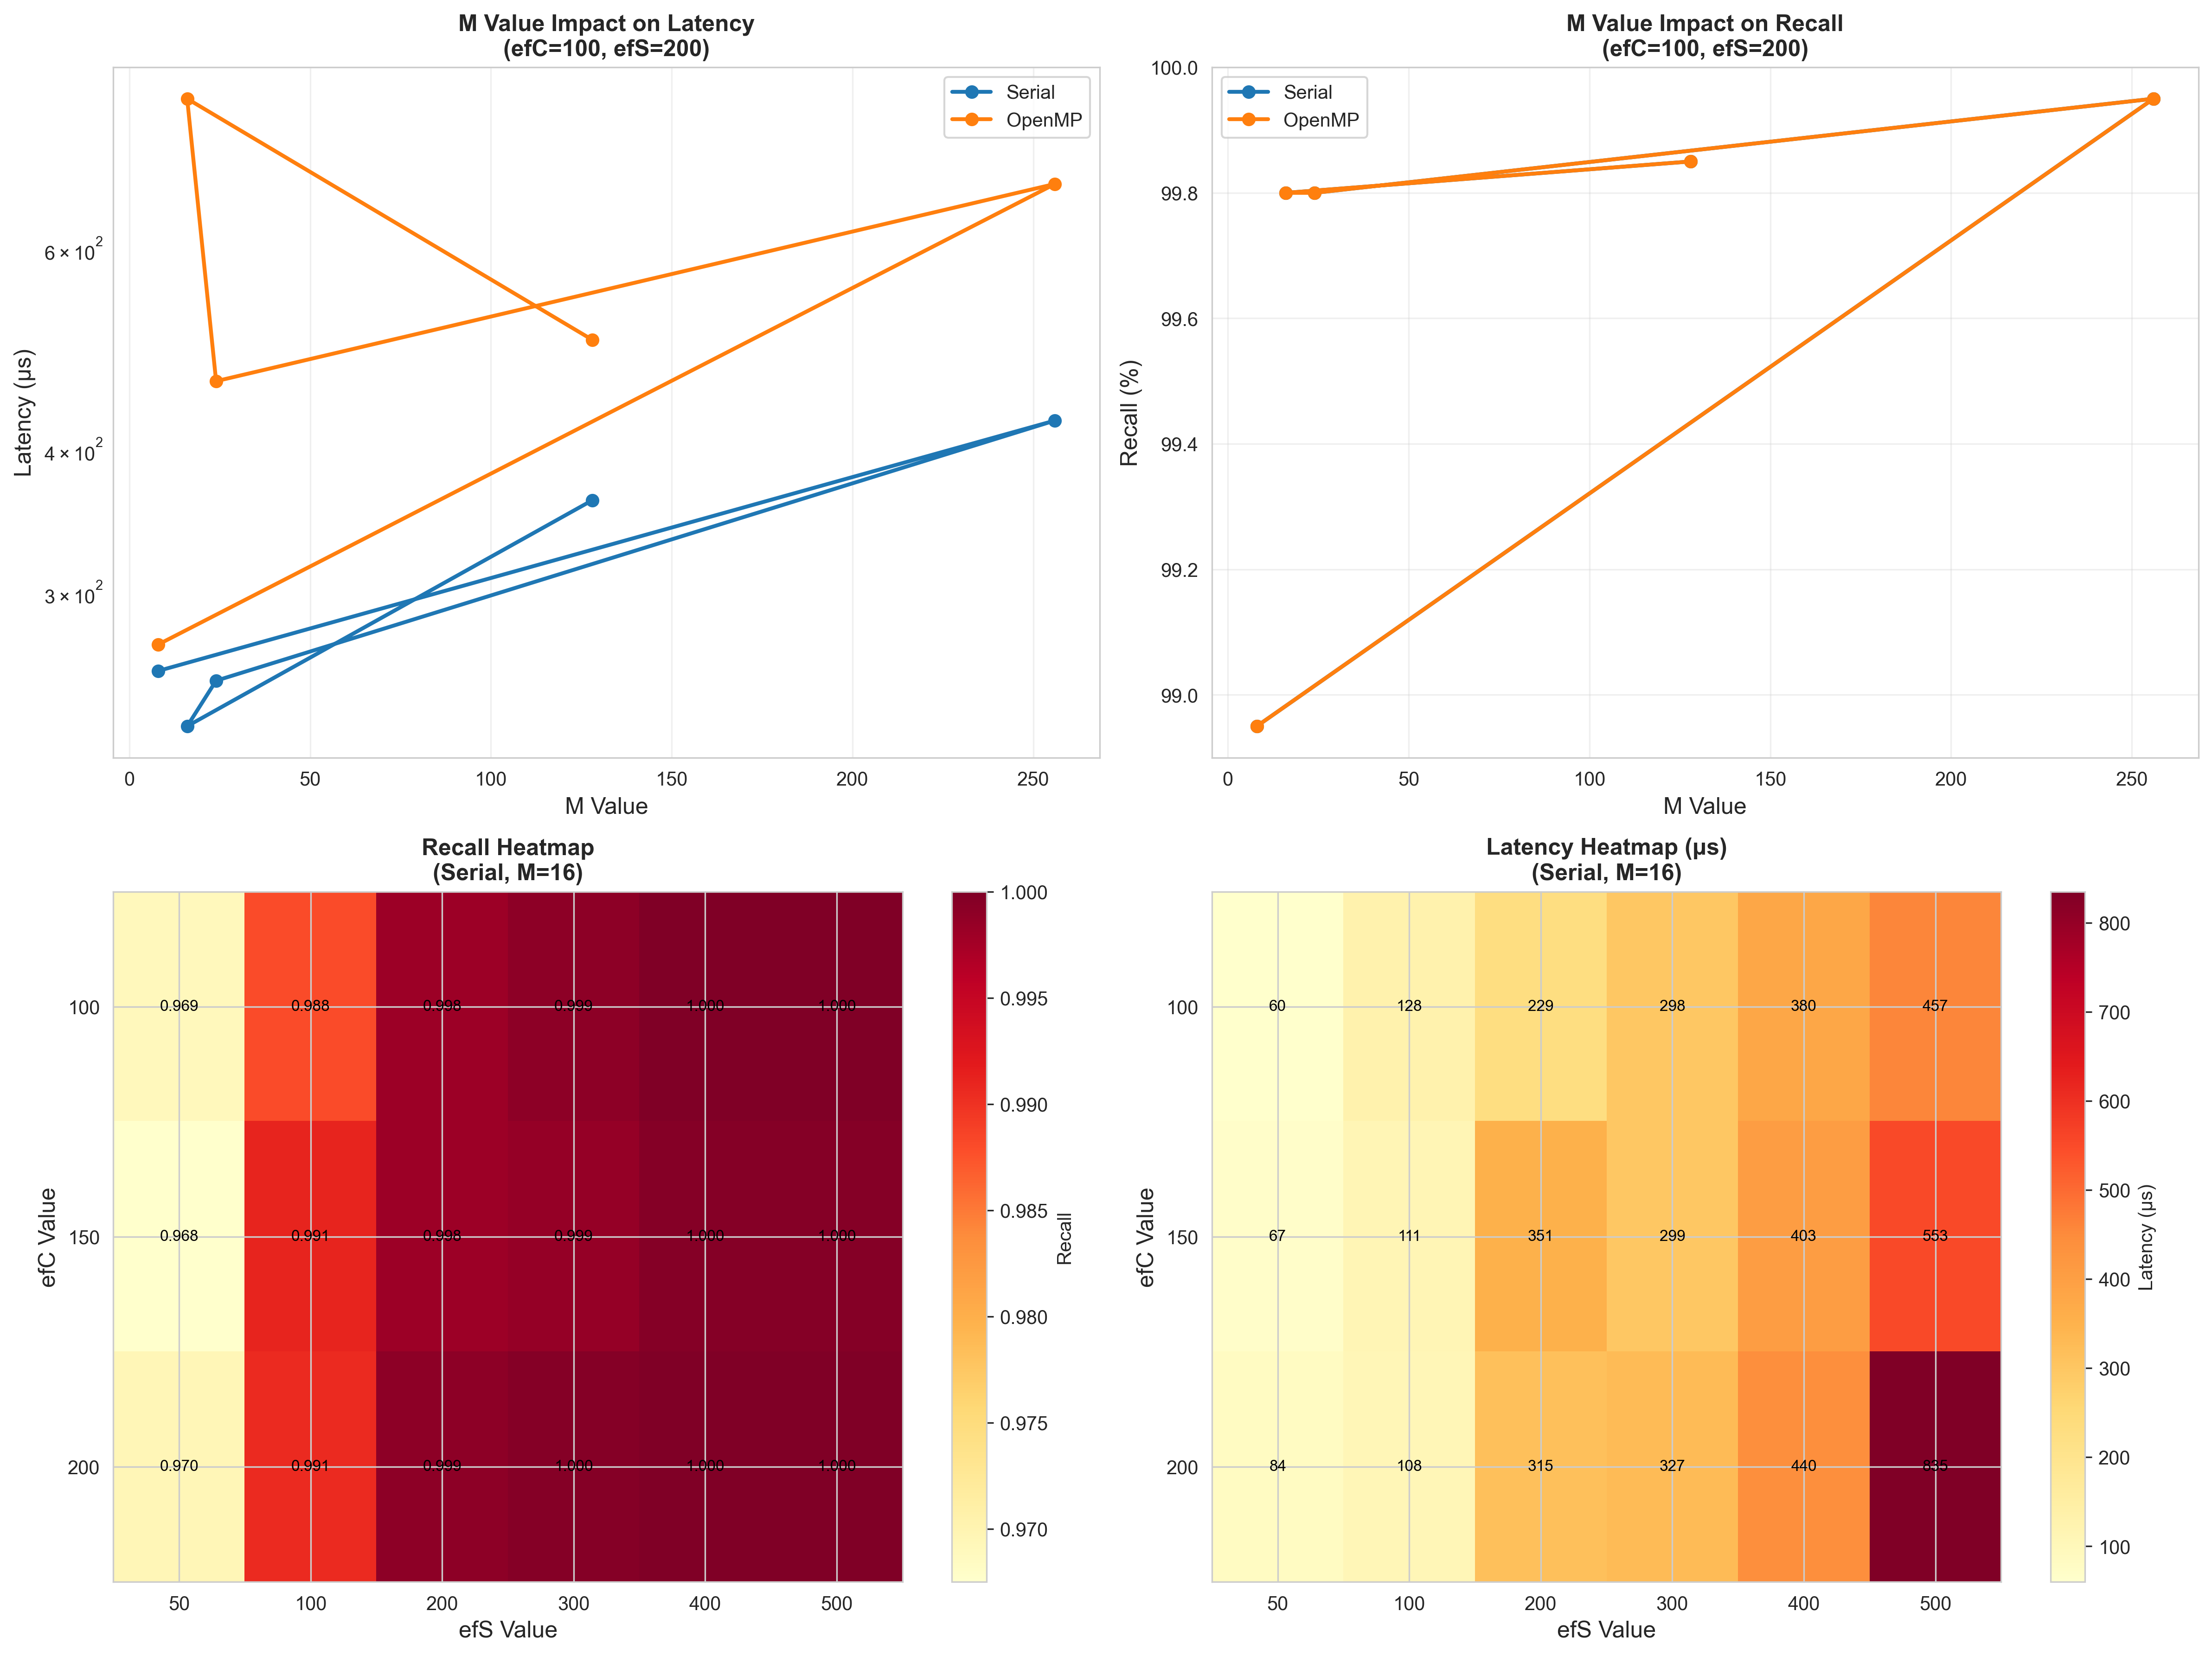
\includegraphics[width=\textwidth]{plots/hnsw_parameter_sensitivity_en.png}
\caption{HNSW算法参数敏感性分析}
\label{fig:hnsw_parameter_sensitivity}
\end{figure}

\paragraph{最优配置推荐}

基于实验结果,我们为不同应用场景推荐以下配置:

\textbf{高召回率场景(召回率≥99.9\%):}
\begin{enumerate}
    \item 串行版本:M=16, efC=100, efS=300(召回率=99.90\%,延迟=298μs)
    \item 串行版本:M=16, efC=200, efS=200(召回率=99.90\%,延迟=315μs)
    \item 串行版本:M=16, efC=200, efS=300(召回率=99.95\%,延迟=327μs)
\end{enumerate}

\textbf{低延迟场景(召回率≥95\%):}
\begin{enumerate}
    \item 串行版本:M=16, efC=100, efS=50(召回率=96.90\%,延迟=60μs)
    \item 串行版本:M=16, efC=150, efS=50(召回率=96.75\%,延迟=67μs)
    \item 串行版本:M=24, efC=100, efS=50(召回率=97.60\%,延迟=70μs)
\end{enumerate}

\subsubsection{多线程实现挑战分析}

HNSW算法的OpenMP并行化效果不佳,主要原因包括:

\begin{enumerate}
    \item \textbf{算法特性限制}:HNSW的搜索过程是一个迭代式的图遍历过程,每一步的搜索方向都依赖于前一步的结果,存在强烈的数据依赖性,难以有效并行化。
    
    \item \textbf{内存访问模式}:图结构的不规则内存访问模式导致缓存命中率低,多线程访问时缓存一致性开销较大。
    
    \item \textbf{线程同步开销}:为保证搜索结果的正确性,需要在关键路径上进行线程同步,增加了额外的开销。
    
    \item \textbf{负载不平衡}:不同层级的搜索复杂度差异很大,导致线程间负载分配不均匀。
\end{enumerate}

\subsubsection{多线程优化总结}

基于实验结果,我们得出以下结论:

\begin{enumerate}
    \item \textbf{HNSW算法不适合简单的OpenMP并行化}:由于算法本身的特性,OpenMP并行化不但没有带来性能提升,反而造成了显著的性能下降。
    
    \item \textbf{推荐使用串行版本}:在当前的实现下,串行版本提供了最佳的性能表现,建议在实际应用中优先考虑串行实现。
    
    \item \textbf{参数调优的重要性}:通过合理的参数配置(特别是M和efS值),可以在召回率和延迟之间取得良好的平衡。
    
    \item \textbf{需要更高级的并行化策略}:若要实现HNSW的有效并行化,需要考虑更复杂的并行策略,如批量查询并行、数据并行或流水线并行等方法。
\end{enumerate} 